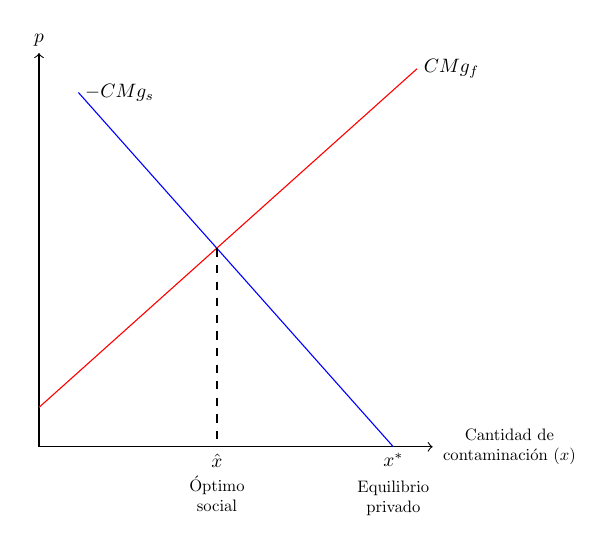
\begin{tikzpicture}
	% Ejes
		\draw[<->] (0,5) node [above, scale=0.7] {$p$}-- (0,0) -- (5,0) node [text width=30mm,text centered, scale=0.6, right] {Cantidad de contaminación $(x)$};
	% Rectas	
		\draw[blue] (0.5,4.5) node [right, scale=0.7, black] {$-CMg_s$} -- (4.5,0) node [below, scale=0.7, black] {$x^\ast$};
		\draw[red] (0,0.5) -- (4.8,4.8) node [right, scale=0.7, black] {$CMg_f$};
	% Línea punteada
		\draw[dashed] (2.26, 2.52) -- (2.26,0) node [below, scale=0.7, black] {$\hat{x}$};
	% Etiquetas
		\draw (2.26,-0.6) node [text width=20mm,text centered, scale=0.6] {Óptimo social};
		\draw (4.5,-0.66) node [text width=25mm,text centered, scale=0.6] {Equilibrio privado};
\end{tikzpicture}